\documentclass[table]{beamer}
\usepackage[german]{babel}

\usepackage{tikz}
\usetikzlibrary{positioning,
                calc,
                decorations.pathreplacing,
                calligraphy}
\usepackage{tikzscale}
\usepackage{libertine}
\usepackage{pgf-pie}
\usepackage{hyperref}
\usepackage{booktabs}
\usepackage{diagbox}
\usepackage{xcolor}
\usepackage{listings}
\lstset{
    backgroundcolor=\color{black},
    basicstyle=\footnotesize,
    basicstyle=\color{white},
    breaklines=true,
    xleftmargin=-2cm,
    framesep=5pt,
    keywordstyle=\color{blue}
}

\title{Versionskontrolle von Texten}
\subtitle{Git und GitHub}
\date{1. Februar 2024}

\begin{document}
    \frame{\titlepage}

    \begin{frame}
        \frametitle{Wichtige Quellen}
        \begin{itemize}
            \item git-scm.com
            \item docs.github.com/decorations
            \item code.visualstudio.com/docs/sourcecontrol/overview
        \end{itemize}
    \end{frame}

    \begin{frame}
        \frametitle{Ausgangslage}
        Wer kennt das nicht?

        \vspace*{5mm}

       \only<2>{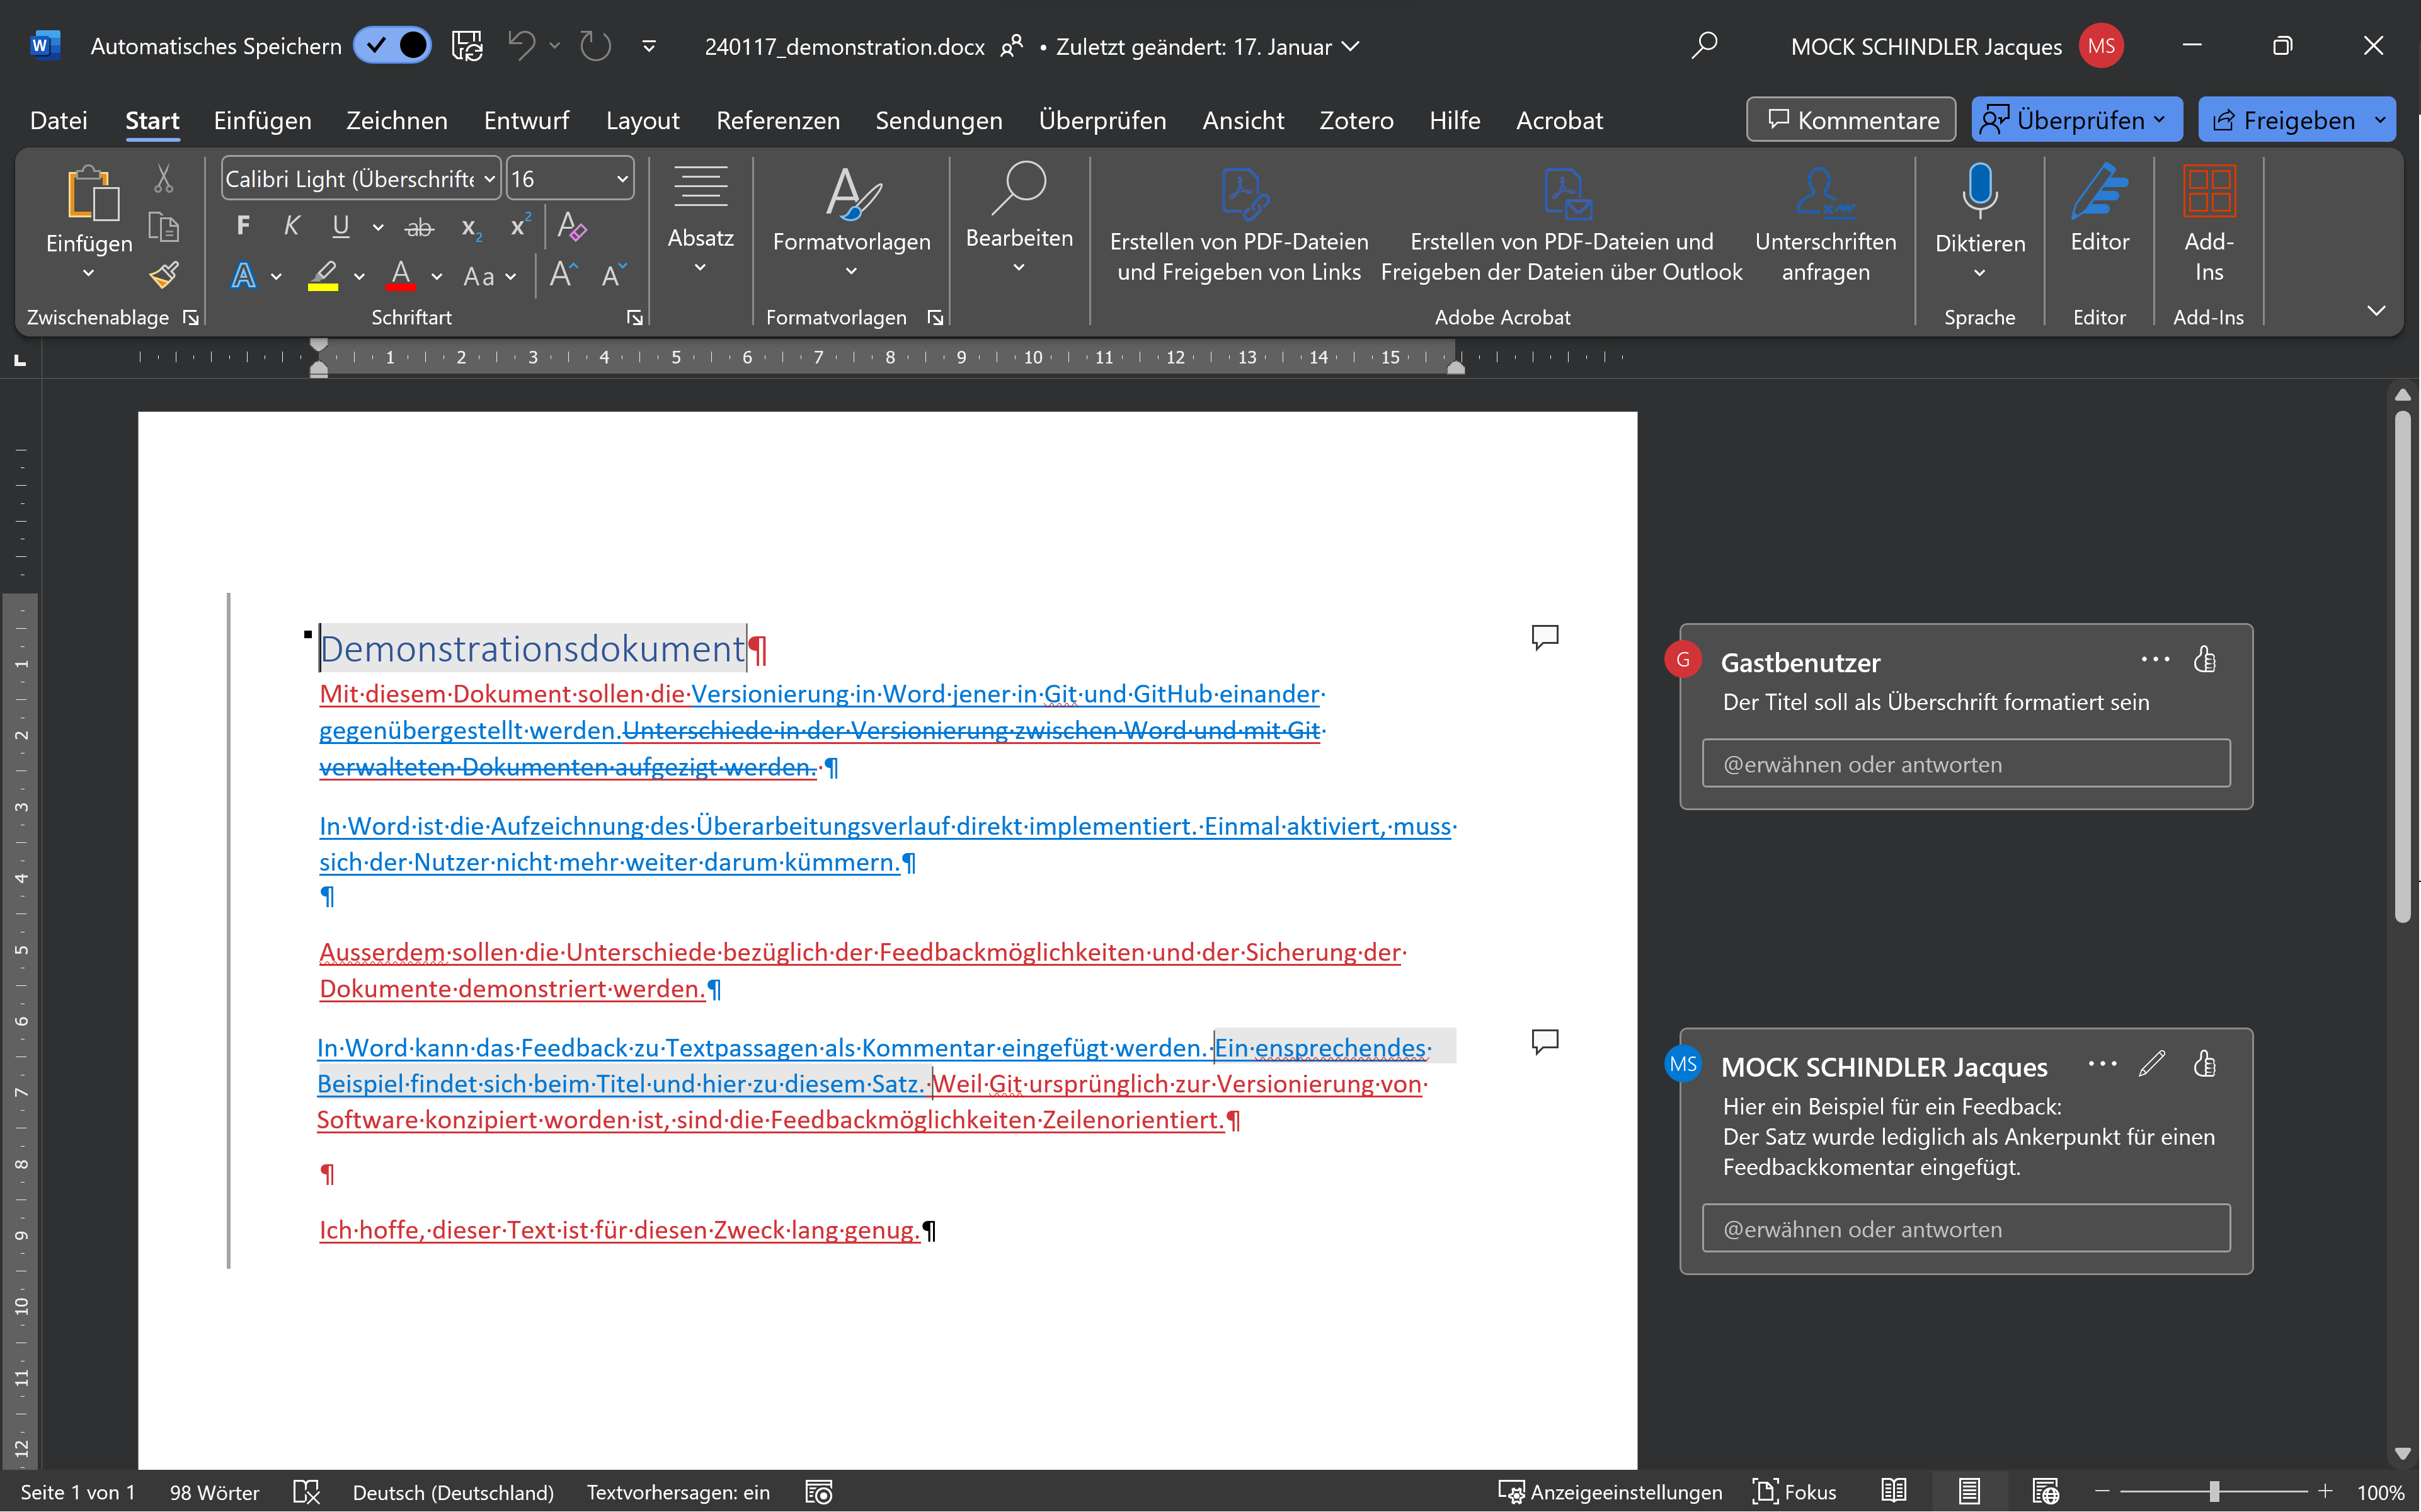
\includegraphics[width=\textwidth]{images/word_markup.png}} 
       \only<3>{
\includegraphics[width=\textwidth]{images/file_manager.png}}
    \end{frame}

    \begin{frame}
        \frametitle{Ausgangslage}
        Das hoffentlich nicht, aber wer weiss?

        \vspace*{5mm}

        \visible<2>{
\includegraphics[width=\textwidth]{images/burning_laptop.png}} 
       
    \end{frame}

    \begin{frame}
        \frametitle{Warum Versionierung}

        \begin{itemize}
            \item Back-up
            \item just one source of truth
            \item transparente Textgenese
        \end{itemize}
    \end{frame}

    \begin{frame}
        \frametitle{Back-up}

        \begin{itemize}
            \item lokales Back-up
                
            nicht so sicher -- insbesondere im Falle eines Velusts des
            Computers
            
           \item Back-up in der Cloud
           
           sicher weil die Daten repliziert sind -- Probleme bietet hier
           allerdings der Datenschutz

           \begin{itemize}
            \item GitHub
            \item GitLab
            \item GitBucket
            \item Azure Repos
            \item \dots
           \end{itemize}
        \end{itemize}   
        
    
    \end{frame}

    \begin{frame}
        \frametitle{Just \textbf{One} Source of Truth}

        \visible<2>{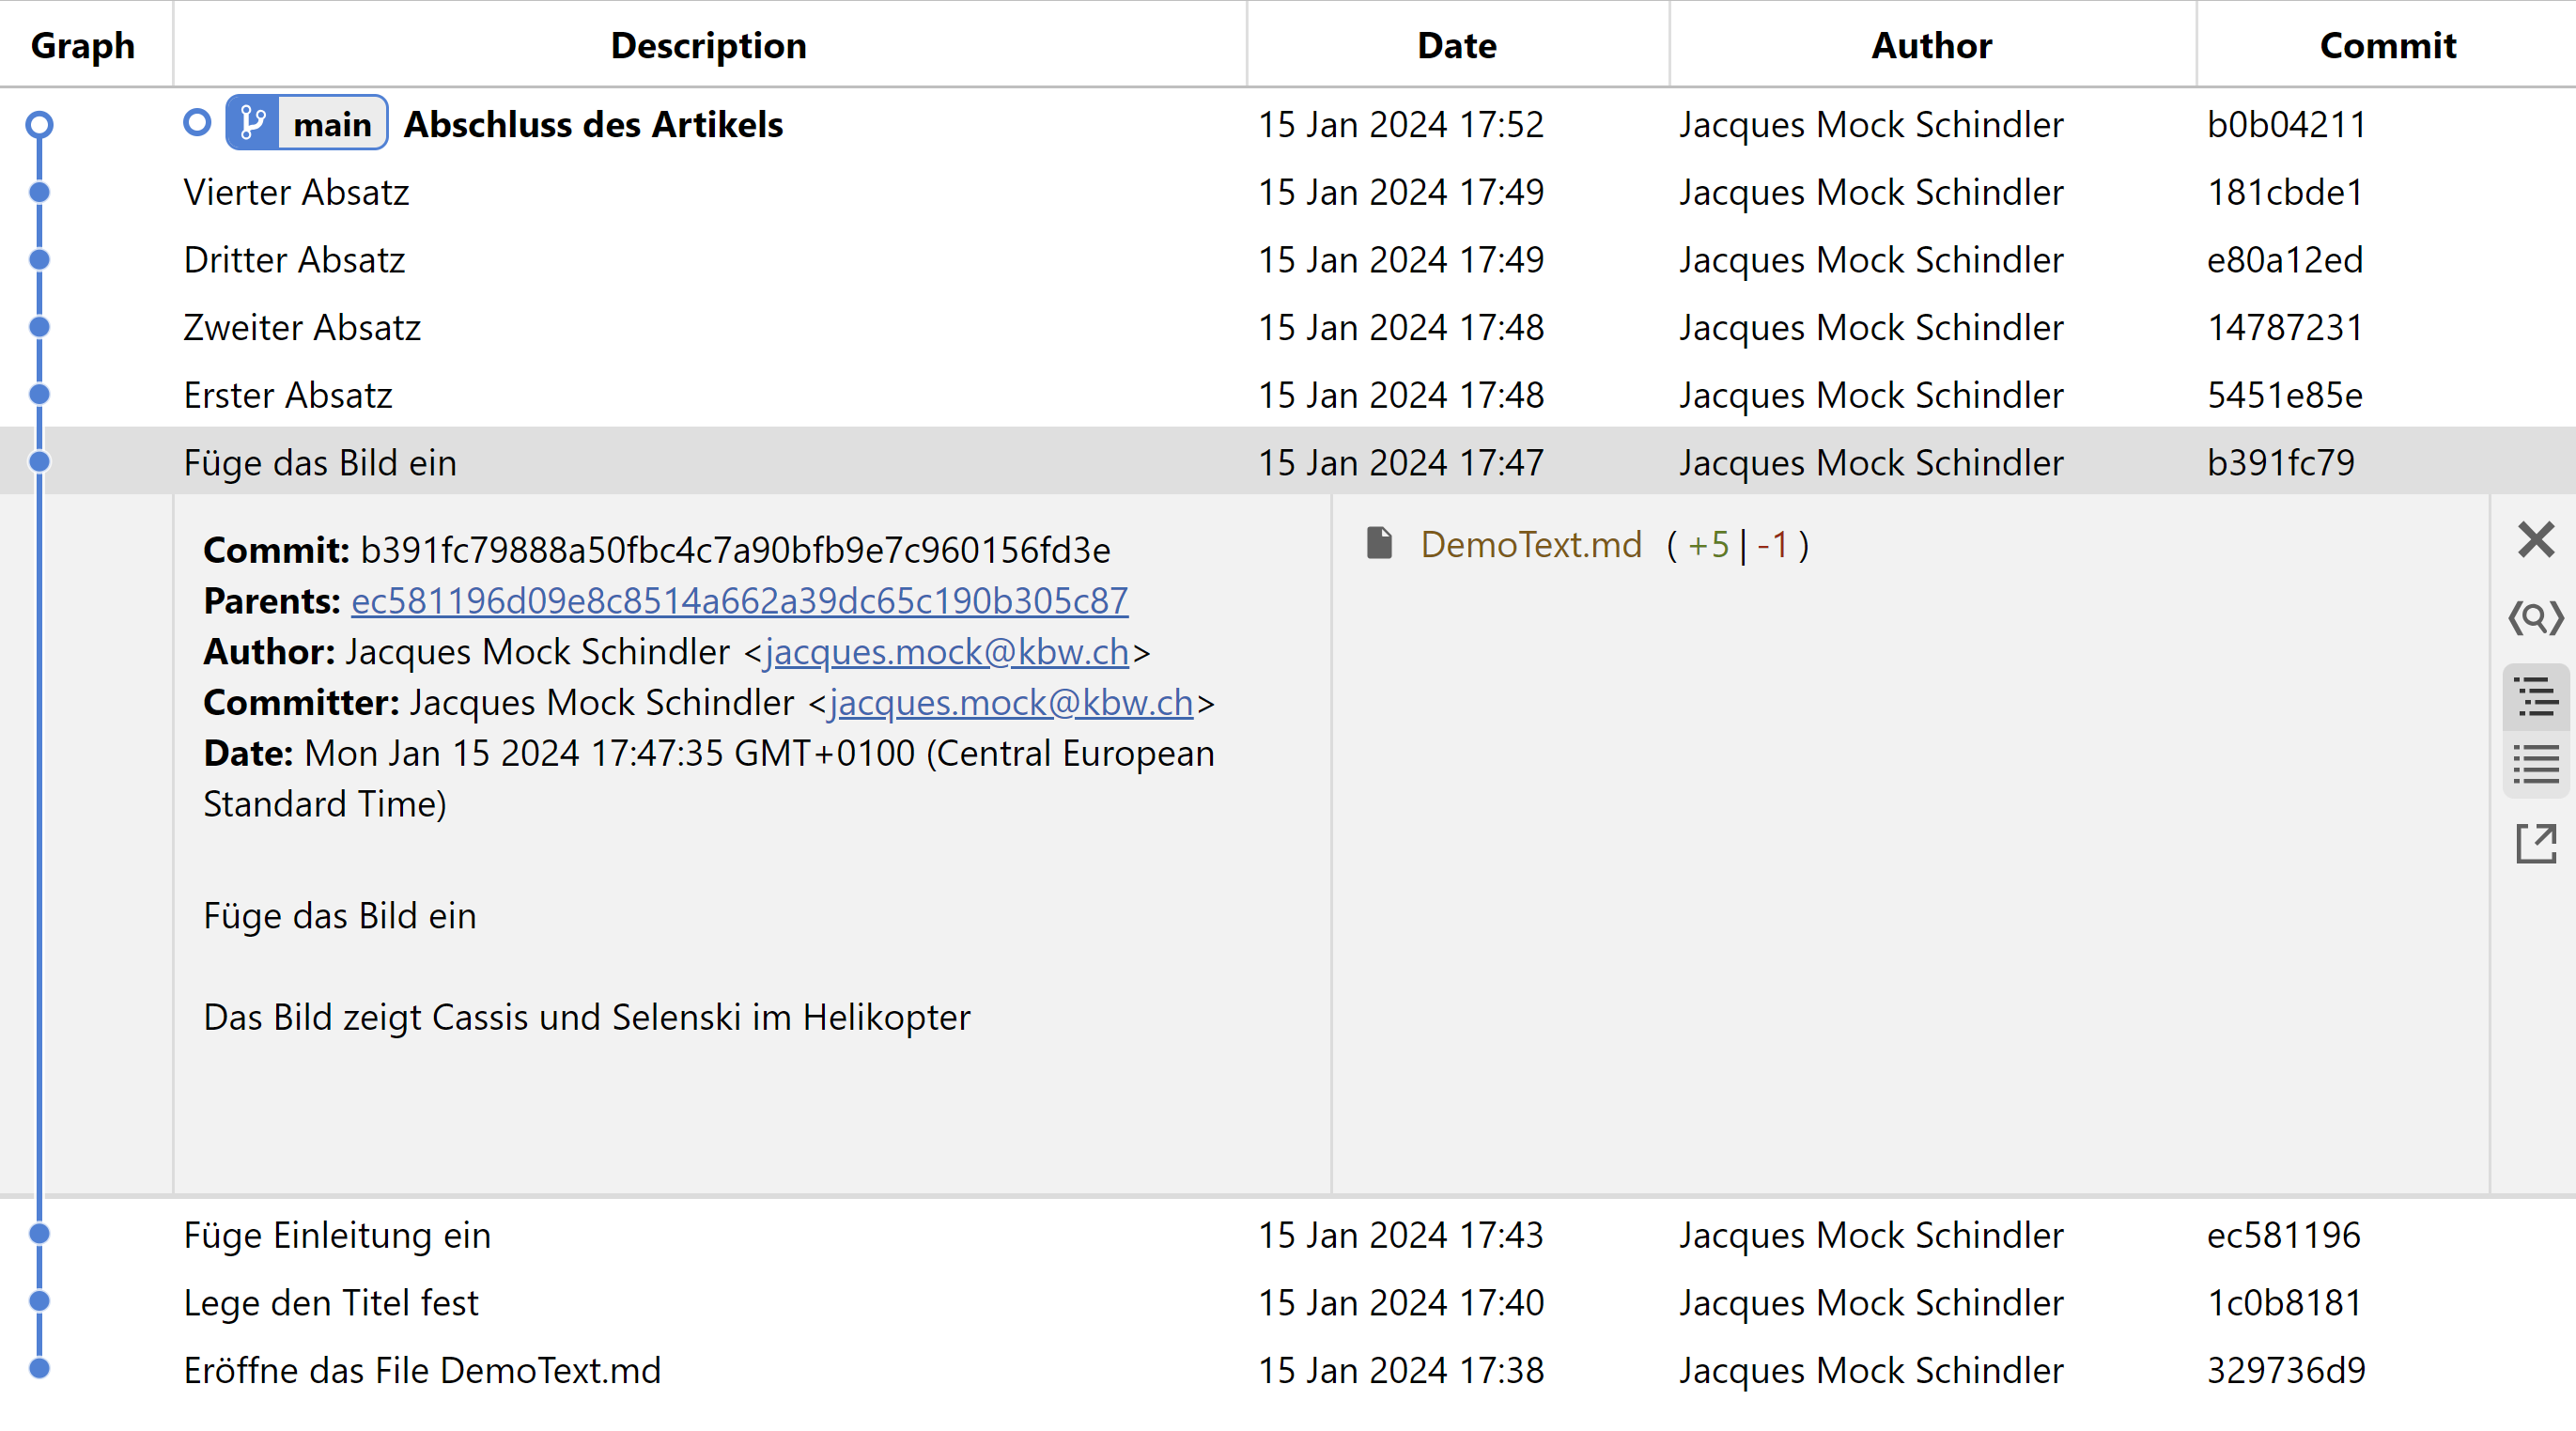
\includegraphics[width=\textwidth]{images/git_graph_details.png}}
    
    \end{frame}

    \begin{frame}
        \frametitle{Transparente Textgenese}

        \visible<2>{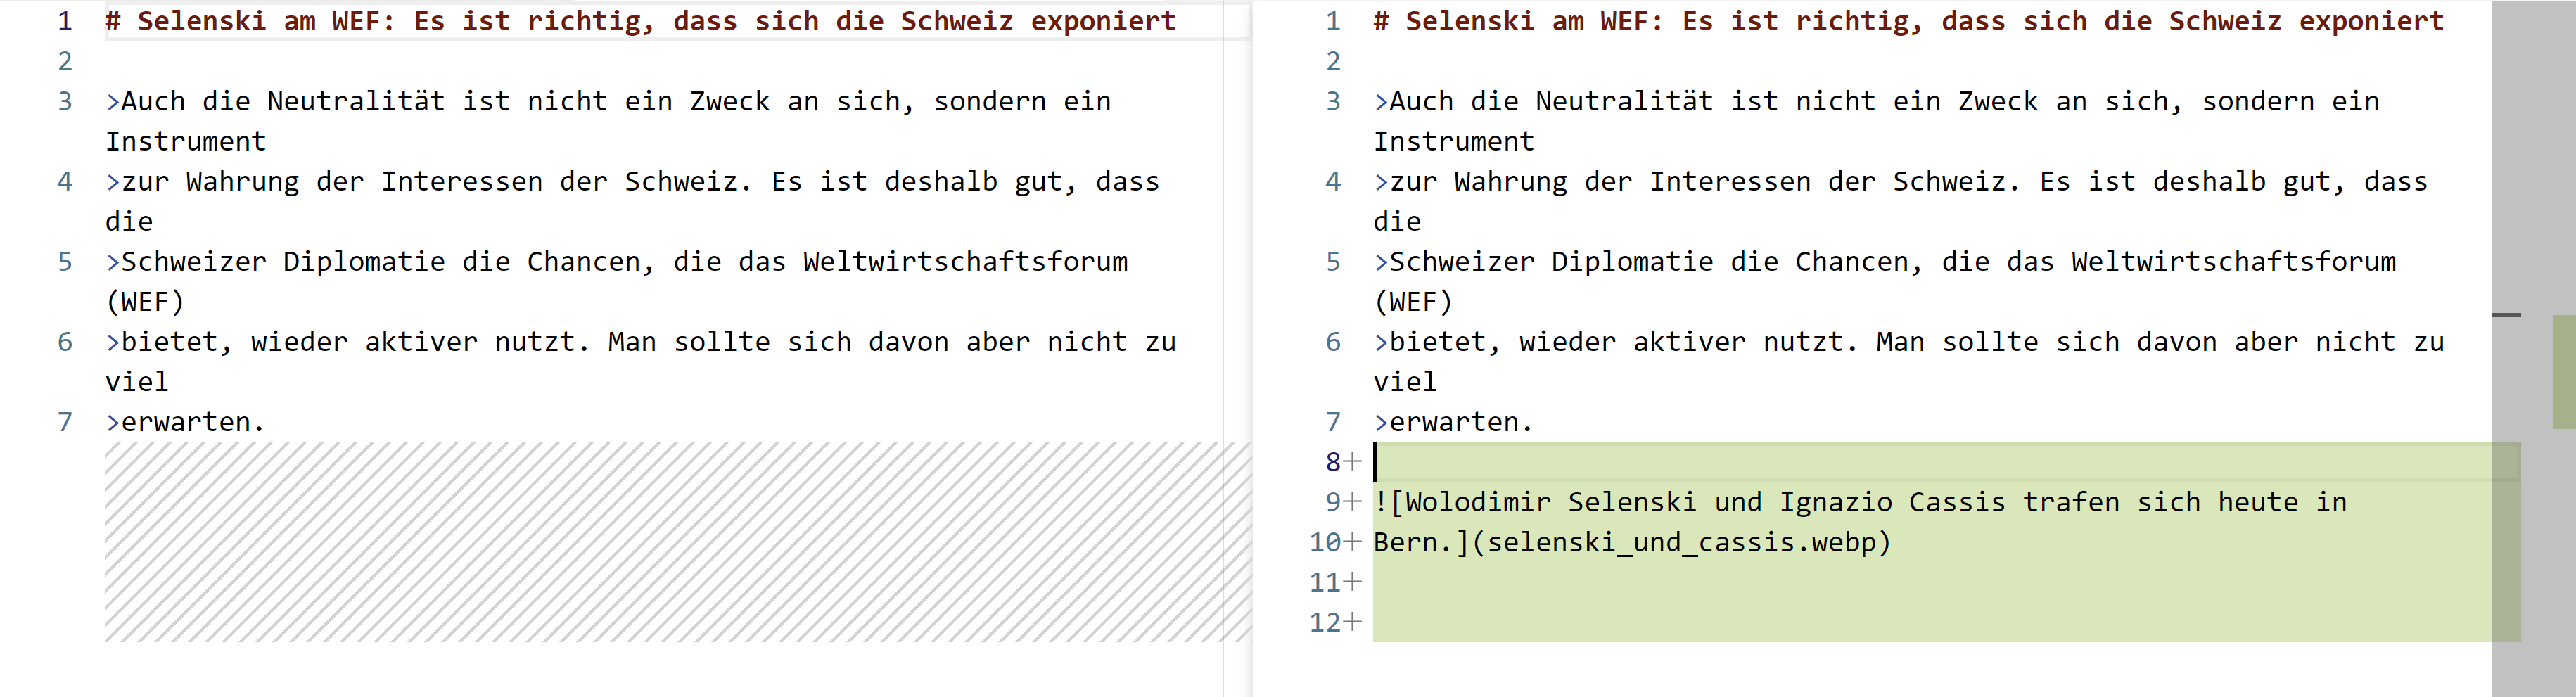
\includegraphics[width=\textwidth]{images/git_graph_aenderung.png}}
    
        
    
    \end{frame}

    \begin{frame}
        \frametitle{Erforderliche Vorbereitungen}

        \begin{itemize}
            \item \textbf{Git (Software)}
            \item GitHub (Konto)
            \item Visual Studio Code (Editor)
            \item pandoc
        \end{itemize}
    
    \end{frame}

    \begin{frame}
        \frametitle{Git}

        \begin{itemize}
            \item Git ist \textbf{die} Versionierungssoftware
            \item Download von git-scm.com 
        \end{itemize}
    
    \end{frame}

    \begin{frame}
        \frametitle{GitHub Konto}

        \begin{itemize}
            \item github.com 
            \item registrieren mit KBW-Identität
        \end{itemize}
    \end{frame}

    \begin{frame}
        \frametitle{Visual Studio Code}

        \begin{itemize}
            \item Editor (nicht erforderlich, aber komfortabel)
            \item Download von code.visualstudio.com/download 
            \item Erweiterung Git Graph (ev. Rewrap, Spell Right, German
            Language Pack for Visual Studio Code)
        \end{itemize}
    
    \end{frame}

    \begin{frame}
        \frametitle{pandoc}

        \begin{itemize}
            \item Format Konverter (nicht erforderlich, aber hilfreich)
            \item Download von pandoc.org/installing.html
        \end{itemize}   
            
    \end{frame}

    \begin{frame}[fragile]
        \frametitle{Mein erstes Projekt}

        Vorbereitung:

        \begin{lstlisting}[language=Bash]
            git config --global user.name = "John Doe"

            git config --global user.email = john.doe@kbw.ch
        \end{lstlisting}  
    
    \end{frame}

    \begin{frame}
        \frametitle{Mein erstes Projekt}

        \only<1,3,5,7>{
            \begin{itemize}
                \item Einloggen auf github.com 
                \item New (grüner Knopf)
                \item Code (grüner Knopf)
                \item Visual Studio Code öffnen
                \item View / Terminal
                \item \texttt{git clone url}
            \end{itemize}
        }

        \only<2>{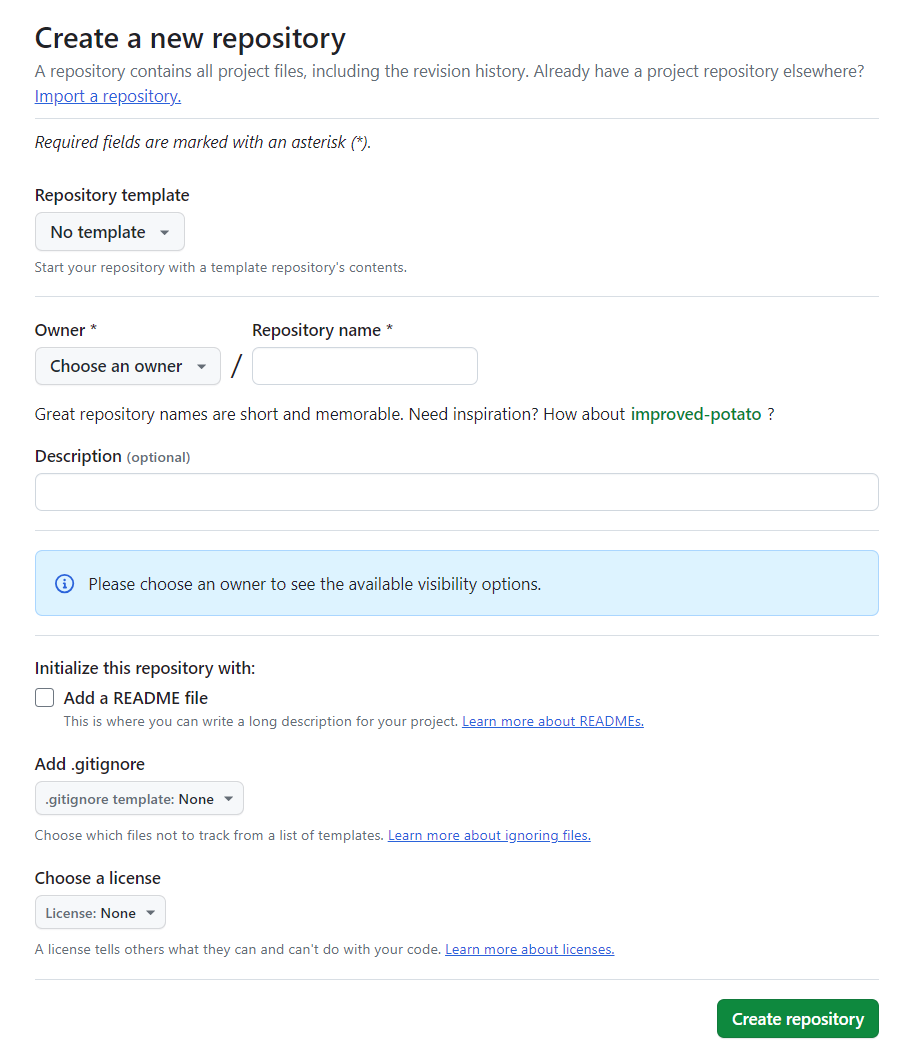
\includegraphics[height=7cm]{images/create_repository.png}}
        \only<4>{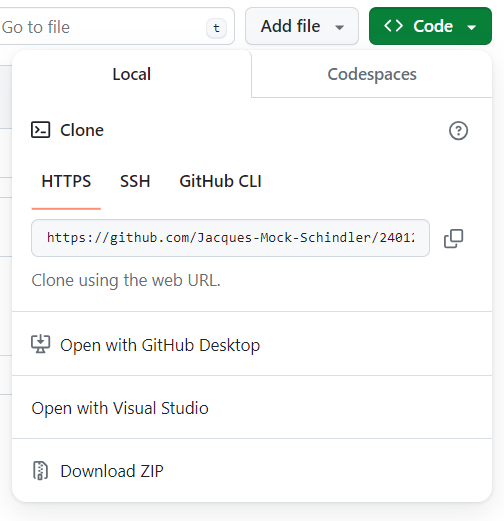
\includegraphics{images/code_button.png}}
        \only<6>{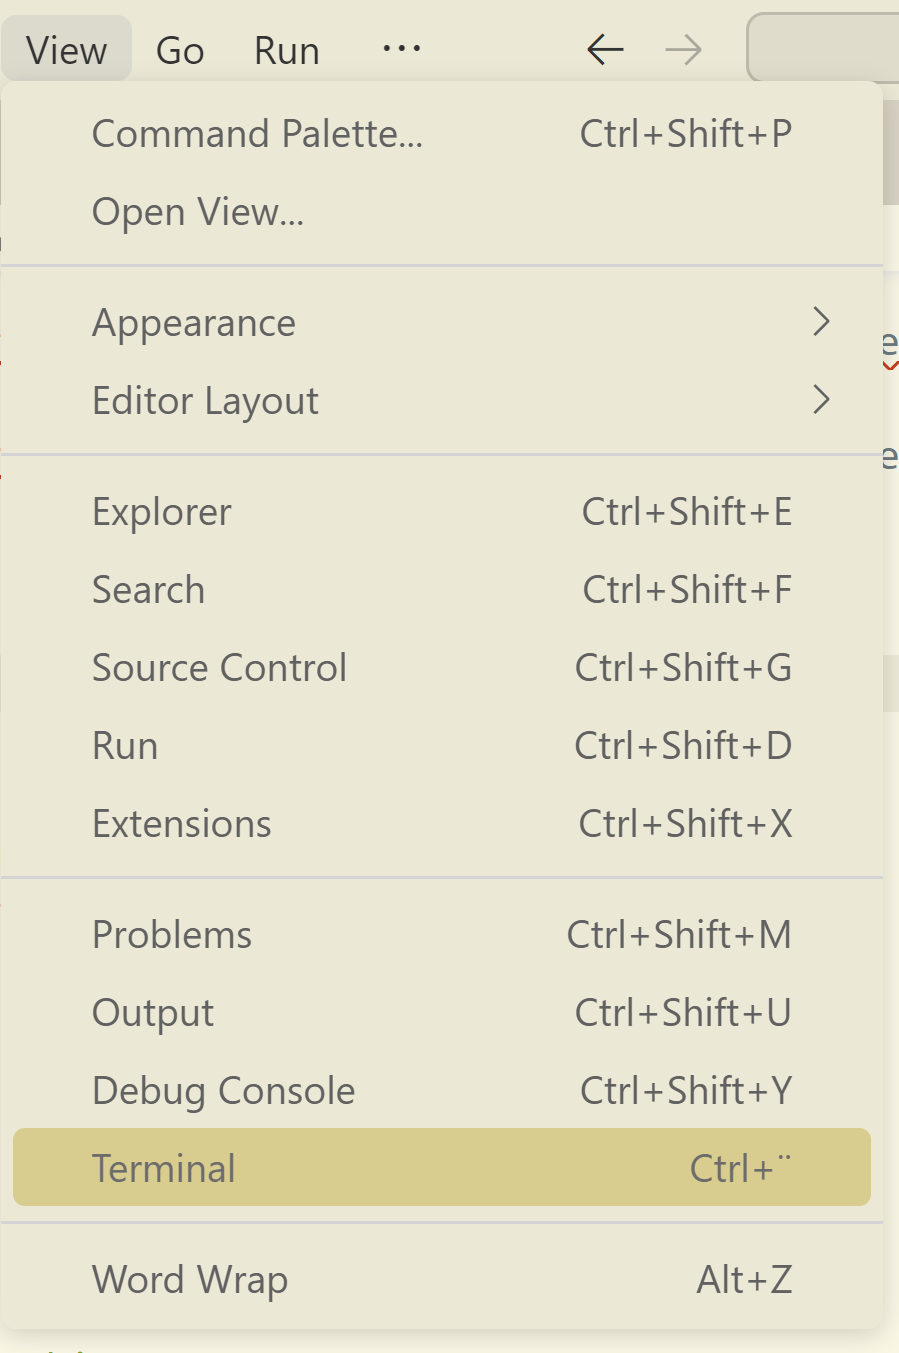
\includegraphics[height=7cm]{images/vsc_view_terminal.png}}      
    
    \end{frame}

    \begin{frame}
        \frametitle{Mein erstes Projekt}

        \only<1,4,6>{
            \begin{itemize}
            \item Schreiben
            \item Commiten
            \item Schreiben
            \item Commiten
            \item Pushen
        \end{itemize}
        }

        \only<2>{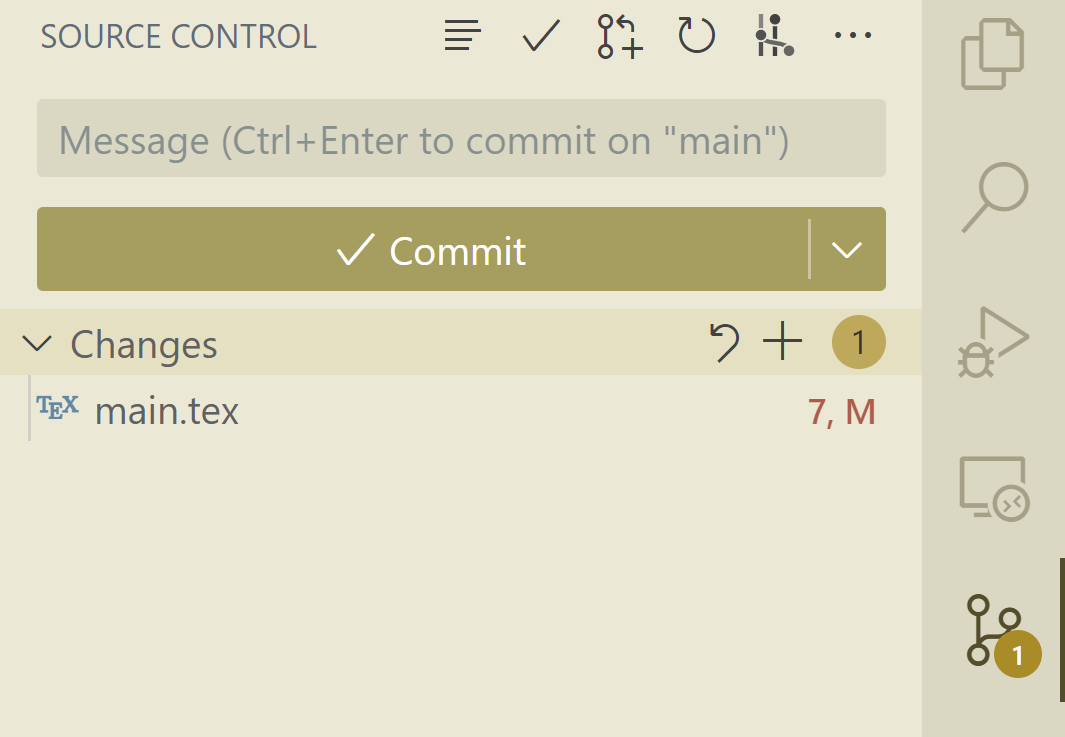
\includegraphics[height=5cm]{images/vsc_commit_window.png}}
        \only<3>{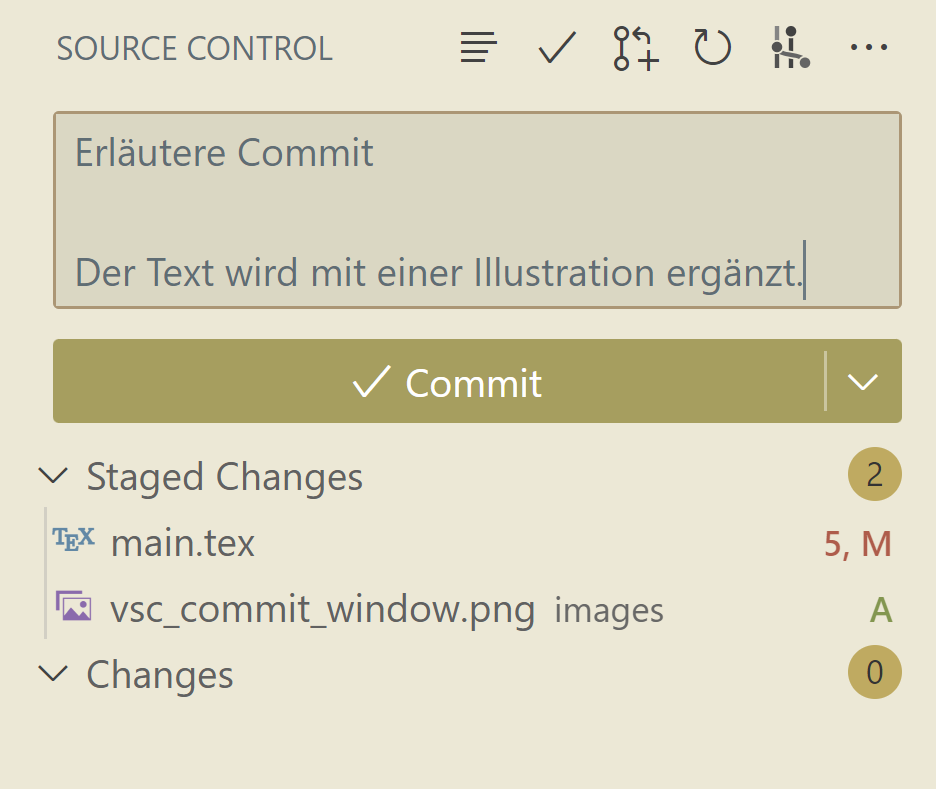
\includegraphics[height=5cm]{images/vsc_commit_message.png}}
        \only<5>{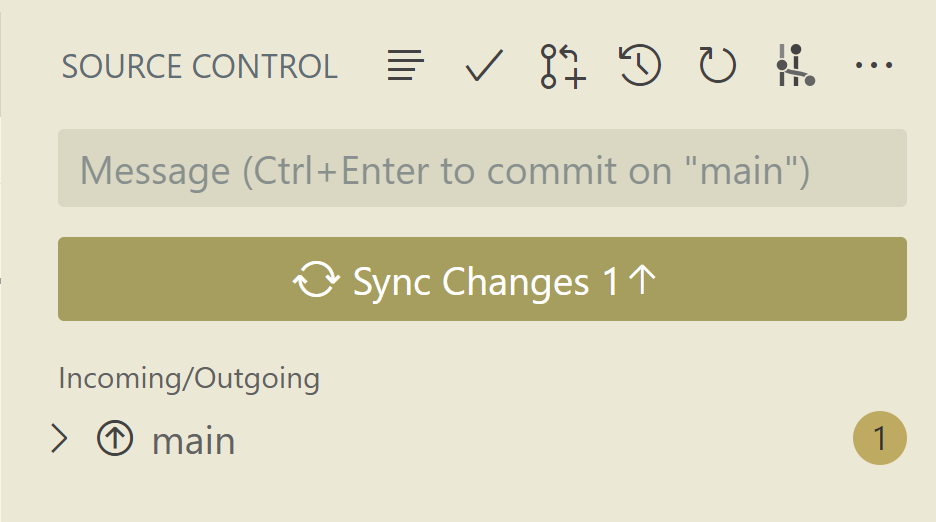
\includegraphics[height=5cm]{images/vsc_push.png}}   
    
    \end{frame}

    \begin{frame}
        \frametitle{Mein erstes Projekt}

        Viel Aufwand -- wozu?

        \begin{itemize}
            \item<2-> transparente Textgenese
            \item<3-> Back-up
            \item<4-> digital Nachhaltig
        \end{itemize}
    
    \end{frame}

    \begin{frame}
        \frametitle{Textvarianten -- Branching}

        \only<1,5>{
            \begin{itemize}
            \item erstellen eines Branches
            \item Schreiben
            \item Commiten
            \item Schreiben
            \item Commiten
            \item Pushen
            \item erstellen eines Pull Requests (Merging)
        \end{itemize}
        }

        \only<2>{
\includegraphics[width=3cm]{images/vsc_branch_indicator.png}}
        \only<3>{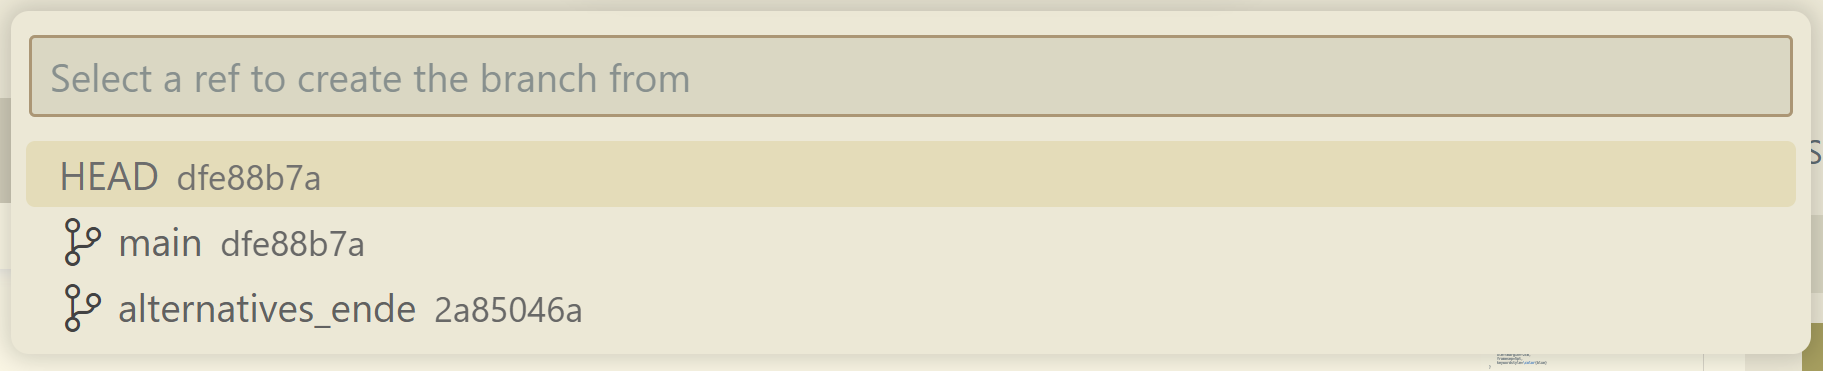
\includegraphics[width=7cm]{images/vsc_branch_auswahl.png}}
        \only<4>{
\includegraphics[width=7cm]{images/vsc_branch_voila.png}}
        \only<6>{
\includegraphics[width=5cm]{images/vsc_pr_button.png}}
        \only<7>{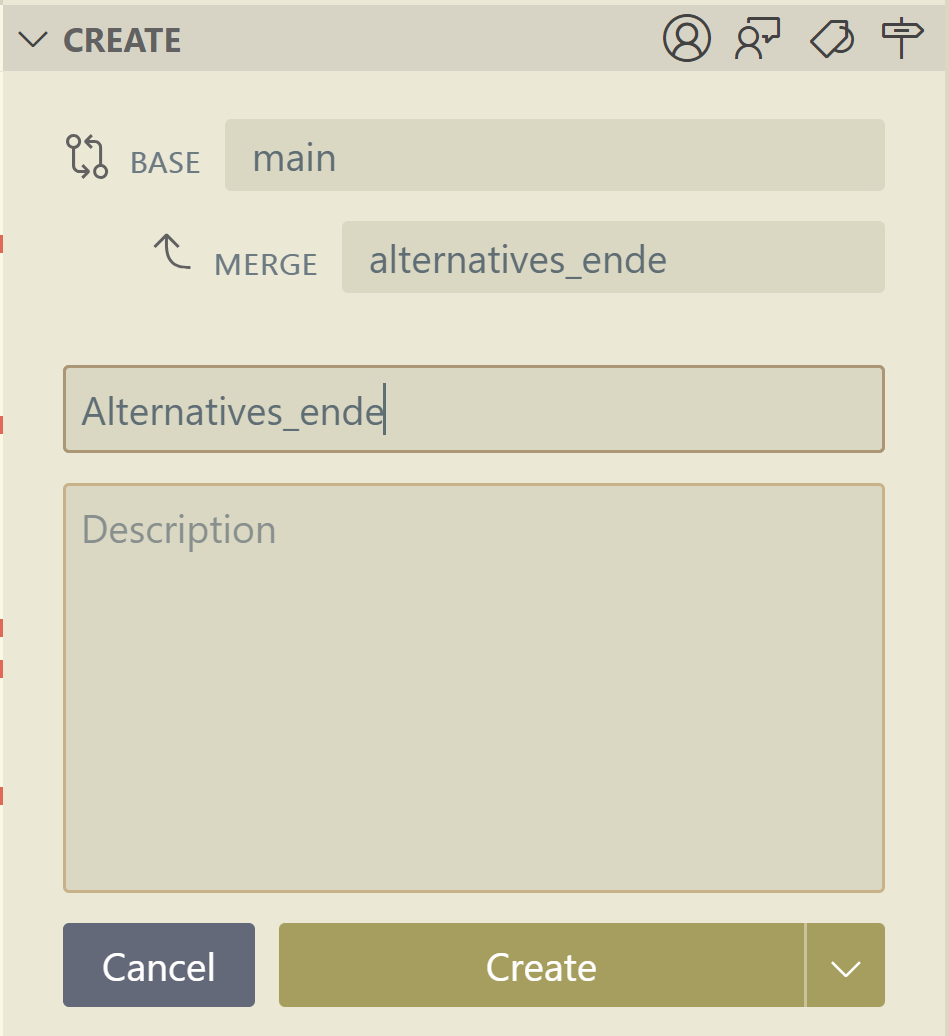
\includegraphics[height=5cm]{images/vsc_pr_dialog.png}}
        \only<8>{
\includegraphics[width=7cm]{images/vsc_merge_dialog.png}}

        
    
        
    
    \end{frame}

    
    \begin{frame}
        \frametitle{Danke}

        \begin{center}
            Just do ist!
        \end{center}
    
    \end{frame}    
    
    



\end{document}
